\documentclass[11pt]{article}


	%
	% Packages and settings for mimicking the Jupyter notebook's behavior
	%
	% \setcounter{secnumdepth}{0} %Suppress section numbers
	%\usepackage{parskip} % Stop auto-indenting (to mimic markdown behaviour)
	% \usepackage{longtable} % longtable support required by pandoc >1.10
	% \usepackage{booktabs}  % table support for pandoc > 1.12.2
	% \usepackage[inline]{enumitem} % IRkernel/repr support (it uses the enumerate* environment)
	% \usepackage[normalem]{ulem} % ulem is needed to support strikethroughs (\sout)
	%								% normalem makes italics be italics, not underlines
	%
	%

	% The hyperref package gives us a pdf with properly built
	% internal navigation ('pdf bookmarks' for the table of contents,
	% internal cross-reference links, web links for URLs, etc.)
	\usepackage{hyperref}
	% The default LaTeX title has an obnoxious amount of whitespace. By default,
	% titling removes some of it. It also provides customization options.
	\usepackage{titling}

	\usepackage{geometry} % Used to adjust the document margins
	\usepackage{textcomp} % defines textquotesingle

	\usepackage{parskip} % omit tab at the beginning of a new paragraph
	\usepackage{upquote} % Upright quotes for verbatim code

	% Figures and styles
	\usepackage[Export]{adjustbox} % Used to constrain images to a maximum size
	\usepackage{float}
	\floatplacement{figure}{H} % forces figures to be placed at the correct location
	\usepackage{graphicx} % Basic figure setup
	\usepackage{fancyvrb} % verbatim replacement that allows latex
	\usepackage{grffile} % extends the file name processing of package graphics 

	% Math
	\usepackage{amsmath} % Equations
	\usepackage{amssymb} % Equations
	\usepackage{mathrsfs}
	\usepackage[mathletters]{ucs} % Extended unicode (utf-8) support


%%
%% BEGIN DOCUMENT
%%
\begin{document}

	%% TODO this should be title and subtitles
	\section{Squared grid puzzle}
	\subsubsection{An informal analysis of the classical nine-dots puzzle	``under steroids''}

	\begin{figure}[H]
		\centering
		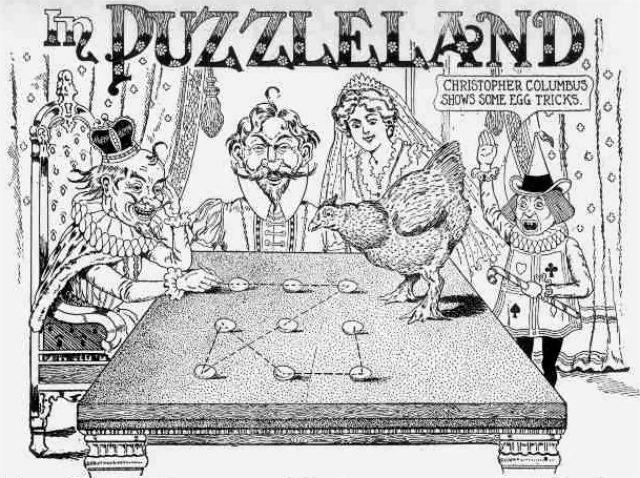
\includegraphics[width=0.5\textwidth]{images/egg_puzzle.jpg}
		\caption{The original illustration of the nine-dots puzzle in the Sam Loyd's "Cyclopedia of puzzle" (1914)}
	\end{figure}

	\hypertarget{introduction} {
		\section{Introduction}
		\label{introduction}
	}
	The \textbf{nine dots puzzle} has been first cited by Sam Loyd's in its
	1914 \emph{Cyclopedia of Puzzles} (see image above). This intriguing
	conundrum was later revived by psychologists, salesmen and ``business
	coaches'' becoming a mainstream \textbf{``thinking-outside-the-box''}
	brain-teaser, i.e.~a benchmark of creative divergent thinking.

	In its basic formulation, the goal is to join nine dots arranged in a
	squared grid with the fewest number of straight lines, and without
	lifting the pen.
	\begin{figure}[H]
	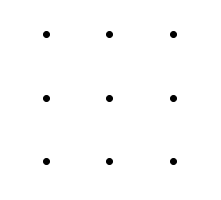
\includegraphics[width=0.2\textwidth]{images/9-dots-grid.png}
	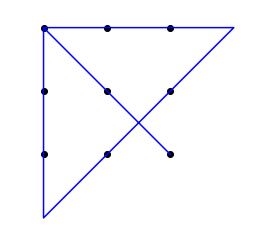
\includegraphics[width=0.2\textwidth]{images/9-dots-solution.png}
	\end{figure}
	The basic version of the puzzle is very famous so you can easily learn
	more about it by searching online, e.g.~you can start from the
	\href{https://en.wikipedia.org/wiki/Thinking_outside_the_box}{Wikipedia
	page}.

	In this paper, I'll discuss a generalized \(2D\) version of the original
	problem, which is extended to a squared grid with an arbitrary number of
	points: the starting \emph{9-dots puzzle} is now the generic
	\emph{9-16-25-36\ldots{} dots puzzle}. First, I'll show that the general
	solution can be drawn iteratively, as one may have already guessed. You
	will also be stunned to learn that, starting from a particular grid size
	upwards, salesmen can no longer refer to the grid problem as a paradigm
	of ``out-of-the-box thinking''. Last but not least, I propose an
	intriguing arithmetical interpretation of the solution for the general
	bidimensional problem.

	\textbf{Disclaimer}: the squared grid problem has already been solved
	and thoroughly treated. Marco Ripà and Pablo Ramirez first extended the
	nine dots problem to a generic \(2D\) squared grid and then also to
	multiple dimensions! You can find their papers in the \hyperlink{references}{References} section.\\
	This document simply aims to be an enjoyable and informal digression on
	the squared grid problem as posed by the aforementioned authors. As
	regards the arithmetical interpretation of the solution to the
	bidimensional puzzle that I'll provide, so far I didn't find any similar
	counterpart by searching online but I may be wrong: in case it's an
	original remark, you're welcome!

	\hypertarget{the-extended-problem-and-its-solution} {
		\section{The extended problem and its solution}
		\label{the-extended-problem-and-its-solution}
	}

	\hypertarget{final-notes}{
		\section{Final notes}
		\label{final-notes}
	}

	\paragraph{Acknowledgements} \mbox{} \\ % mbox needed for having carriage return after "paragraph"
	Marco Ripà posed the squared grid brain-teaser during one of its
	stimulating YouTube live sessions. I am obliged to him for the great fun
	I had in tackling this problem, which in turn inspired all the analysis
	and ideas that followed.

	\paragraph{Technical note} \mbox{} \\
	Python was used to code the generic solver algorithm and produce the
	explanatory images of the paper. You can find the implementation code in
	the attached Jupyter notebook, in which you can also display and save a
	nice animation drawing the solution to the puzzle.

	\paragraph{Future developments} \mbox{} \\
	I'll work on solving the problem in multiple dimensions, you bet! I
	would also like to extend the solver's code to handle this more general
	case; hence, as a plus I could produce animations drawing the solution
	for three-dimensional grids.

	\hypertarget{references}{
		\section{References}
		\label{references}
	}

	\begin{itemize}
		\item
			The basic nine-dots puzzle has been first cited here: \emph{Cyclopedia of Puzzles, Samuel Loyd (1914)}
		\item
			A link to a really valid \href{http://utenti.quipo.it/base5/geopiana/loyd9punti4linee.htm}{online reference (in Italian)}
		\item
			\emph{Marco Ripà and Pablo Ramirez, Il Nine Dots Puzzle esteso a N×N×\ldots×N punti}.
		\item
			\emph{Marco Ripà, Nine Dots Puzzle extended to N1×N2×\ldots×Nk points 	under house arrest}.
	\end{itemize}

\end{document}
